\documentclass[a4paper]{article}
\usepackage{a4wide}
\usepackage[utf8]{inputenc}
\usepackage{amsmath}
\usepackage{mathtools}
\usepackage{amssymb}
\usepackage[english]{babel}
\usepackage{mdframed}
\usepackage{systeme,}
\usepackage{lipsum}
\usepackage{relsize}
\usepackage{caption}
\usepackage{tikz}
\usepackage{tikz-3dplot}
\usetikzlibrary{shapes.geometric}
\usepackage{pgfplots}
\usepackage{pgfplotstable}
\pgfplotsset{compat=newest}%1.7}
\usepackage{harpoon}%
\usepackage{graphicx}
\usepackage{wrapfig}
\usepackage{subcaption}
\usepackage{authblk}
\usepackage{float}
\usepackage{listings}
\usepackage{xcolor}
\usepackage{chngcntr}
\usepackage{amsthm}
\usepackage{comment}
\usepackage{commath}
\usepackage{hyperref}%Might remove, adds link to each reference
\usepackage{url}
\usepackage{calligra}

%\usepackage[backend=biber]{biblatex}
%\addbibresource{refs.bib}

% Commands

\newcommand{\w}{\omega}
\newcommand{\curl}[1]{\mathbf{\nabla}\times \mathbf{#1}}
\newcommand{\grad}{\mathbf{\nabla}}
\newcommand{\dive}[1]{\mathbf{\nabla}\cdot \mathbf{#1}}
%\newcommand{\crr}{\mathfrak{r}}
\newcommand{\res}[2]{\text{Res}(#1,#2)}
\newcommand{\laplace}{\nabla^2}
\newcommand{\trace}{\text{Tr}}
\newcommand{\fpartial}[2]{\frac{\partial #1}{\partial #2}}
\newcommand{\rot}[3]{\begin{vmatrix}\hat{x}&\hat{y}&\hat{z}\\\partial_x&\partial_y&\partial_z\\#1&#2&#3 \end{vmatrix}}
\newcommand{\newparagraph}{\vspace{.5cm}\noindent}

% Special character commands
\DeclareMathAlphabet{\mathcalligra}{T1}{calligra}{m}{n}
\DeclareFontShape{T1}{calligra}{m}{n}{<->s*[2.2]callig15}{}
\newcommand{\crr}{\mathcalligra{r}\,}
\newcommand{\boldscriptr}{\pmb{\mathcalligra{r}}\,}



\title{FK8028: Two particles interacting}
\author{Author: Andreas Evensen}
\date{Date: \today}
\definecolor{codegreen}{rgb}{0,0.6,0}
\definecolor{codegray}{rgb}{0.5,0.5,0.5}
\definecolor{codepurple}{rgb}{0.58,0,0.82}
\definecolor{backcolour}{rgb}{0.95,0.95,0.92}

\lstdefinestyle{mystyle}{
    backgroundcolor=\color{backcolour},   
    commentstyle=\color{codegreen},
    keywordstyle=\color{magenta},
    numberstyle=\tiny\color{codegray},
    stringstyle=\color{codepurple},
    basicstyle=\ttfamily\footnotesize,
    breakatwhitespace=false,         
    breaklines=true,                 
    captionpos=b,                    
    keepspaces=true,                 
    numbers=left,                    
    numbersep=5pt,                  
    showspaces=false,                
    showstringspaces=false,
    showtabs=false,                  
    tabsize=2
}

\lstset{style=mystyle}

\begin{document}

\maketitle
\pagenumbering{Roman}
\newpage
\pagenumbering{roman}
\setcounter{page}{1}
\newpage
\tableofcontents
\newpage
\pagenumbering{arabic}
\section{Introduction}
In this report one investigates the behavior of two particles interacting with a Lennard-Jones potential. The time-integration is computed in accordance to a method called Velocity Verlet (Verlet Method) which allows for computing a particles position in time as a function of velocity and acceleration.
With two different initial conditions one observes different behavior. When two particles are placed close to the equilibrium distance, the particles start to oscillate with the resonance frequency of the system. 
When placed tightly together, the atoms repel each-other and overcomes the potential barrier and escapes the potential field.

\newparagraph
The integration method used is also said to be symplectic, which is found to be true where one finds that the energy is conserved for small enough time-steps when placing the particles close to the equilibrium distance. 


\section{Theoretical background and method}
This section will introduce the necessary theory for the problem at hand, and the method used to solve the problem.
\subsection{Theory}
Given a system of $N$ particles, where each interact with each-other via some potential $\mathcal{V}(\mathbf{r_i}, \mathbf{r}_j)$, one defines the total potential energy of the system as:
\begin{align*}
    V(\mathbf{r}_i) = \sum_{j=1, j\neq i}^N \mathcal{V}(\mathbf{r}_i, \mathbf{r}_j),
\end{align*}where $i$ and $j$ represent the index of the particles. Given this, one can reduce the dimension of the system by allowing the system to contain only two particles, which interact with each other via some potential $\mathcal{V}(\mathbf{r}_i, \mathbf{r}_j)$. In this paper, the potential is defined as the interatomic potential, also known as the Lennard-Jones potential, given by:
\begin{align}
    \mathcal{V}(\mathbf{r}_1, \mathbf{r}_2) &= 4\epsilon\left(\left(\frac{\sigma}{\abs{\mathbf{r}_1 - \mathbf{r}_2}}\right)^{12} - \left(\frac{\sigma}{\abs{\mathbf{r}_1 - \mathbf{r}_2}}\right)^6\right). \label{eq: LJ Potential}
\end{align}This interaction gives rise to a force between the particles, which is given by:
\begin{align}
    \mathbf{F}(\mathbf{r}_1, \mathbf{r}_2) &= -\grad{\mathcal{V}} = 4\epsilon\left(12\left(\frac{\sigma}{\abs{\mathbf{r}_1 - \mathbf{r}_2}}\right)^{12} - 6\left(\frac{\sigma}{\abs{\mathbf{r}_1 - \mathbf{r}_2}}\right)^6 \right)\frac{\mathbf{r}_1 - \mathbf{r}_2}{\abs{\mathbf{r}_1 - \mathbf{r}_2}^2},\label{eq: LJ Force}
\end{align}where $\epsilon$ is the so-called dispersion energy, in magnitude of electron volts, and $\sigma$ is the size of the particle, in magnitude of Ångström[1]. 
In this paper, the particles are Argon atoms, which yields $\epsilon = 0.0103$~eV and $\sigma = 3.4$~Å. The force between the particles can also be expressed by a forward difference method of the potential:
\begin{align}
    \mathbf{F} &= -\grad{\mathcal{V}} \approx \frac{\Delta \mathcal{V}}{\Delta x}\hat{x} + \frac{\Delta \mathcal{V}}{\Delta y}\hat{y} + \frac{\Delta \mathcal{V}}{\Delta z}\hat{z}, \label{eq: Difference force}
\end{align}

\newparagraph
The system is treated as a classical system, where the particles are treated as point particles. The kinetic energy of the system is then defined as:
\begin{align*}
    \mathcal{K}(t) &= \sum_i \frac{m_i\mathbf{\mathbf{v}_i(t)}^2}{2}\\
    &=\sum_i \frac{\mathbf{p}_i^2}{2m_i},
\end{align*}where $m_i$ is the mass of the particle, $\mathbf{v}_i$ is the velocity, and $\mathbf{p}_i$ is the momentum of the i:th particle.
From this one can then define the Hamiltonian of the system $\mathcal{H}(t)$ as:
\begin{align}
    H(t) &= \sum_i \dot{\mathbf{q}}_i\mathbf{p}_i + V(\{\mathbf{q}_i\}), \label{eq: Hamiltonian}
\end{align}where $\mathbf{q}_i$ and $\mathbf{p}_i$ is the velocity and momentum of particle $i$ respectively.

\subsection{Method}
In this paper one investigates how the particles' trajectory evolves in time, and how the energy of the system evolves in time.
This is done via the Velocity Verlet method[2], defined as:
\begin{align}
    \mathbf{r}_i(t + dt) &= \mathbf{r}_i(t) + \mathbf{v}_i(t) + \frac{1}{2}\mathbf{a}_i(\mathbf{r}_i(t))dt^2,\label{eq: Pos Verlet}\\
    \mathbf{v}_i(t + dt) &= \mathbf{v}_i(t) + \frac{dt}{2}\left[\mathbf{a}_i(\mathbf{r}_i(t + dt)) + \mathbf{a}_i(\mathbf{r}(t))\right].\label{eq: Vel Verlet}
\end{align}
In the above numerical scheme, $\mathbf{r}_i$ is the position, $\mathbf{v}_i$ is the velocity and $\mathbf{a}_i$ is the acceleration of the i:th particle. Note that the velocity of the next position is dependent on the acceleration of that time-step.
The algorithm structure is given by:
\begin{enumerate}
    \item Initialize the position and velocity of the particles.
    \item Compute the acceleration of the particles.
    \item Compute the position of the particles according to eq \eqref{eq: Pos Verlet}.
    \item Compute the new acceleration of the particles given the updated positions
    \item Compute the velocity of the particles according to eq \eqref{eq: Vel Verlet}.
    \item Updated the time with the time-step.
    \item Go back to step 2 and repeat until the desired time is reached. 
\end{enumerate}
The method is a symplectic method which means that the energy of the system is conserved[3]. This is a very important property to have in a simulation of this type, as it simulate a physical system.

\newparagraph
The Verlet method is a forth order accurate method, which means that the error is of order $\mathcal{O}(dt^4)$[2]. This is a very good property to have in a numerical scheme, as it allows for a large time-step, while still maintaining a good accuracy.
However, the method is not stable for all time-steps, and thus one will have to find the absolute stability condition for the method. 
Furthermore, the scales of the system is typically very small. As mentioned previously the scales of the system is in magnitude of Ångström, which means that one will have to scale the system to a more manageable scale.
In order to do this one has to find appropriate units to work with: $dt = ~[\text{ps}]$, $m = ~[\text{eVs}^2/\text{Å}^2]$, $r = ~[\text{Å}]$, $v = ~[\text{Å/s}]$, $F = ~[\text{eV/Å}]$.
The timescale of the system is in pico-seconds which is due to the fact that the system is in magnitude of Ångström.

\newpage
\section{Result \& Discussion}

The interatomic potential, eq \eqref{eq: LJ Potential}, and the force, eq \eqref{eq: LJ Force}, is plotted in figure \ref{fig: Interatomic potential and force}.
\begin{figure}[H]
    \centering
    \begin{subfigure}[b]{0.45\textwidth}
        \centering
        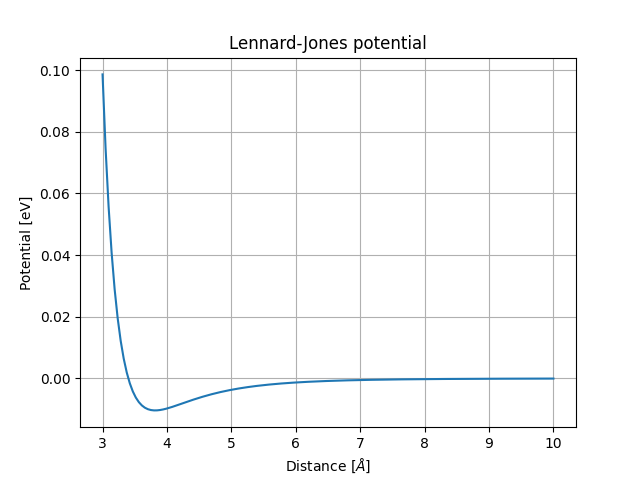
\includegraphics[width=\textwidth]{Lennard-Jones potential.png}
        \caption{Lennard-Jones potential $\mathcal{V}(\mathbf{r})$}
        \label{fig: Interatomic potential}
    \end{subfigure}
    \hfill
    \begin{subfigure}[b]{0.45\textwidth}
        \centering
        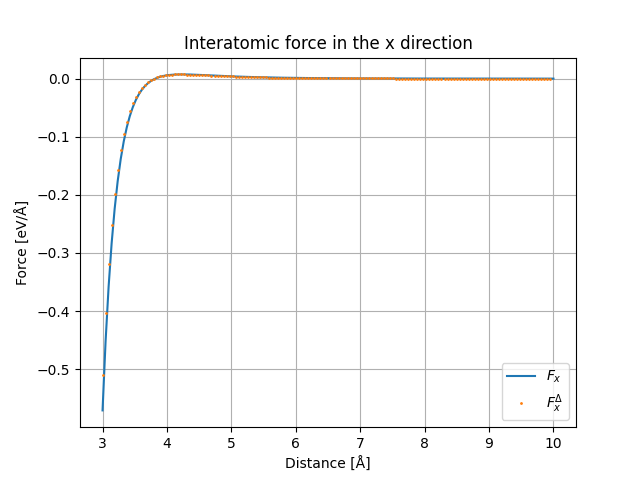
\includegraphics[width=\textwidth]{Interatomic force in the x direction.png}
        \caption{Force interaction in the $\hat{x}$ direction.}
        \label{fig:Interatomic force}
    \end{subfigure}
    \caption{Lennard-Jones potential and force.}
    \label{fig: Interatomic potential and force}
\end{figure}\noindent
The potential, fig \ref{fig: Interatomic potential}, shows the potential experienced between to atoms as a function of distance between them. The potential has a minimum at $\abs{\mathbf{r}} \approx 3.8$~Å which corresponds to the equilibrium distance between the atoms.
The force, fig \ref{fig:Interatomic force}, shows the force experienced between two atoms as a function of distance between them. The force is zero at the equilibrium distance. The force grows exponentially as the distance between the atoms decreases. 

\subsection{Trapped atoms}
Two Argon atoms are placed at a distance $4$~Å apart, and in time the atoms starts to oscillate around the equilibrium distance $\abs{\mathbf{r}} \approx 3.8$~Å. This is seen in figure \ref{fig: Position}.
The two atoms velocities alternate in direction and magnitude, which is the result of the oscillatory behavior of the position. This is seen in figure \ref{fig: Velocity}.

\begin{figure}[H]
    \centering
    \begin{subfigure}[b]{0.45\textwidth}
        \centering
        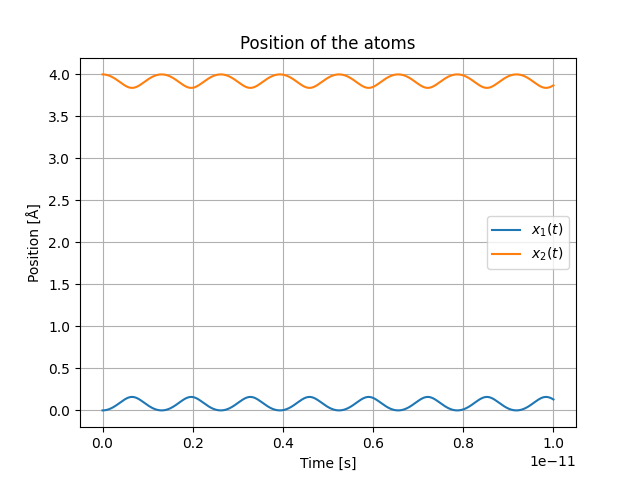
\includegraphics[width=\textwidth]{Position of the atoms.png}
        \caption{Position as a function of time $x(t)$ for the two atoms.}
        \label{fig: Position}
    \end{subfigure}
    \hfill
    \begin{subfigure}[b]{0.45\textwidth}
        \centering
        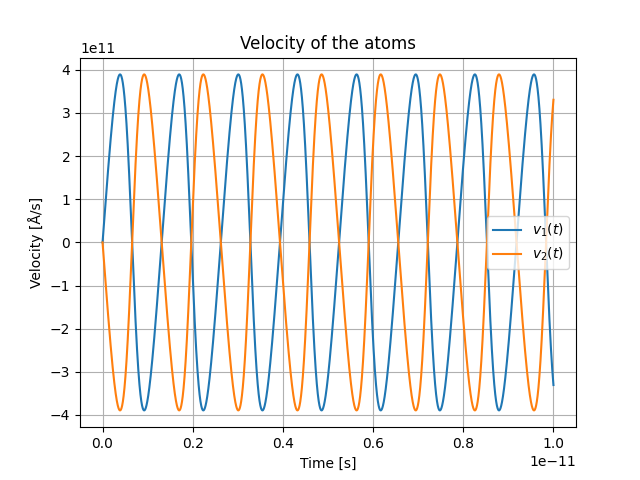
\includegraphics[width=\textwidth]{Velocity of the atoms.png}
        \caption{Velocity as a function of time $v_x(t)$ for the two atoms.}
        \label{fig: Velocity}
    \end{subfigure}
    \caption{The atoms position and velocity as a function of time.}
    \label{fig: Position & Velocity}
\end{figure}\noindent
The equilibrium distance $r_{\text{eq}}$ can be computed according:
\begin{align*}
    r_{\text{eq}} &= 2^{1/6}\sigma \approx 3.816\text{ Å},
\end{align*}which is in agreement with the equilibrium distance found in figure \ref{fig: Position} where the equilibrium distance is $\abs{\mathbf{r}} \approx 3.8$~Å.
The oscillations that occur in figure \ref{fig: Position} occur with a frequency[1]:
\begin{align*}
    f \approx \frac{3}{4\cdot 10^{-11}}~\left[\frac{1}{\text{s}}\right] = 750 \text{ GHz}.
\end{align*}This frequency corresponds to the natural frequency of an $\text{Ar}_2$ molecule, which is the result of the Lennard-Jones potential, eq \eqref{eq: LJ Potential}.

\newparagraph
The system is governed by the Hamiltonian, eq \eqref{eq: Hamiltonian}, which is plotted in figure \ref{fig: Energy of the atoms} alongside the total kinetic energy $\mathcal{K}(t)$ and the potential energy $\mathcal{V}(t)$.
One can see that the Hamiltonian of the system $\mathcal{H}(t)$ is constant in type, which implies that the energy is conserved throughout the simulation.

\begin{figure}[H]
   \centering
   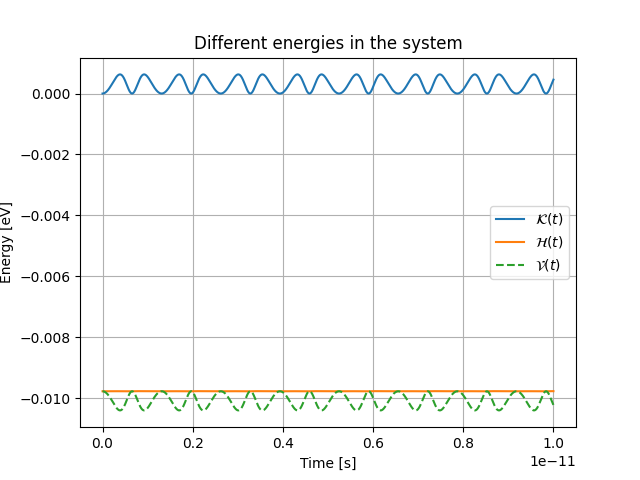
\includegraphics[scale = 0.55]{Different energies in the system.png} 
   \caption{Various energies as a function of time for the system.}
   \label{fig: Energy of the atoms}
\end{figure}\noindent
The total energy $E$ of such as a system is conserved in classical mechanics, and thus the only reason for this behavior is the numerical error in the Verlet method and the difference method in computing the velocity, eq \eqref{eq: Vel Verlet}.
The Hamiltonian for different time-steps is plotted in figure \ref{fig: Hamiltonian with different time-steps}. One can see that the Hamiltonian is stable for $dt< 10^{-12}$~s.
This is the result of the Verlet method being a forth order accurate method, which means that the error is of order $\mathcal{O}(dt^4)$.
\begin{figure}[H]
    \centering
    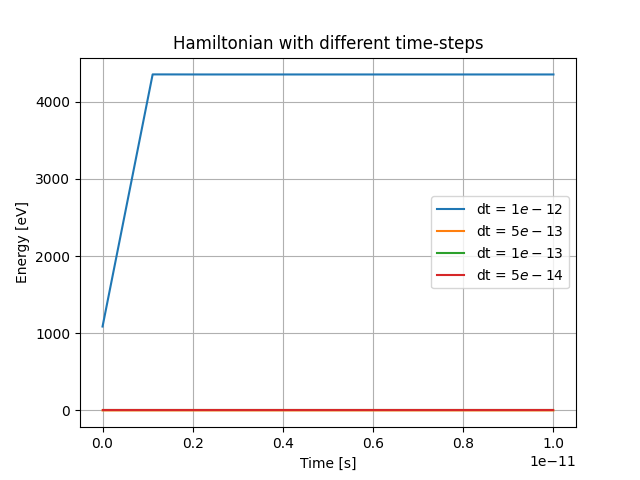
\includegraphics[scale = .5]{Hamiltonian with different time-steps.png}
    \caption{Hamiltonian as a function of time for different time-steps.}
    \label{fig: Hamiltonian with different time-steps}
\end{figure}

\subsection{Escaping atoms}
In the previous section, the atoms were place a distance of $4$~Å apart. In this section one investigates the time-evolution if the Argon atoms are placed a distance $3$~Å apart.
As seen in figure \ref{fig:Interatomic force}, when the relative position is $3$~Å, the atoms repel each-other with a significant force. This can be seen in the below figure, where the position of the two particles is computed as a function of time.
\begin{figure}[H]
    \centering
    \begin{subfigure}[b]{0.45\textwidth}
        \centering
        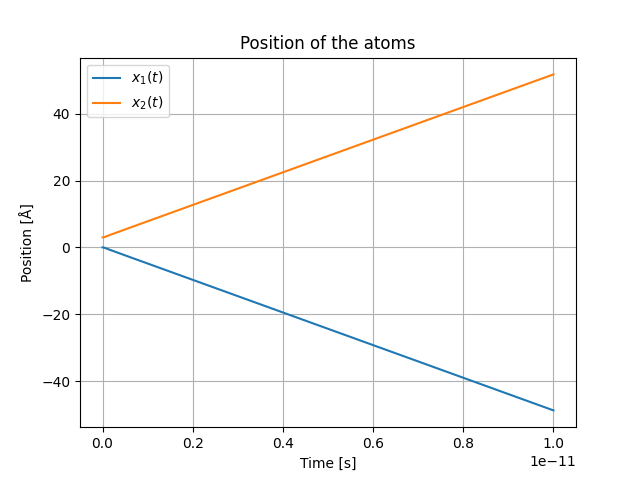
\includegraphics[width=\textwidth]{position_close.png}
        \caption{Position as a function of time $x(t)$ when placed $3$~Å apart.}
        \label{fig: close position}
    \end{subfigure}
    \hfill
    \begin{subfigure}[b]{0.45\textwidth}
        \centering
        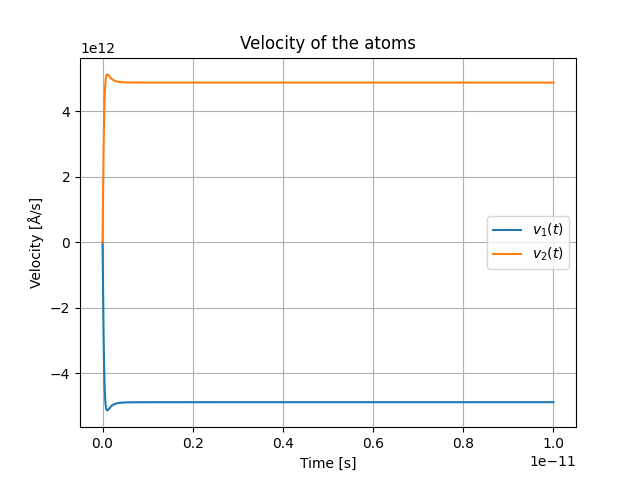
\includegraphics[width=\textwidth]{velocity_close.png}
        \caption{Velocity as a function of time $v_x(t)$ when placed $3$~Å apart.}
        \label{fig: close Velocity}
    \end{subfigure}
    \caption{The atoms position and velocity as a function of time.}
    \label{fig: Position & Velocity close}
\end{figure}\noindent
In figure \ref{fig: close position} the positions show that the two atoms are moving away from each-other after escaping the equilibrium distance.
This can further be seen in figure \ref{fig: close Velocity} where the velocity is constant after a short time. This is because the atoms are at a distance that the force is negligible.
The different energies in the system are shown in figure \ref{fig: close energy}.
\begin{figure}[H]
    \centering
    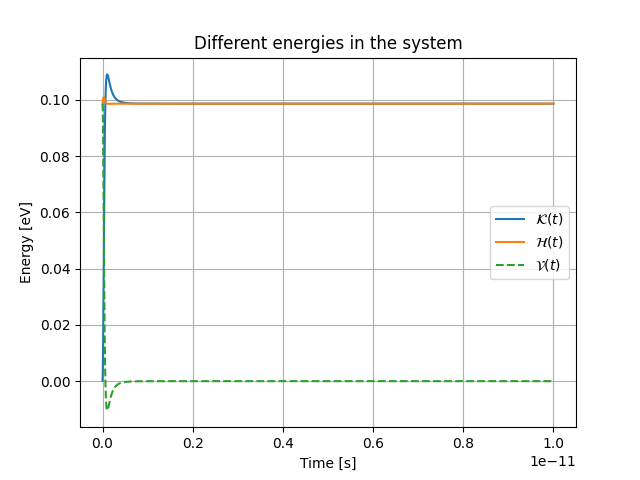
\includegraphics[scale = 0.5]{energies_close.png}
    \caption{Energies of the system when initially placed $3$~Å apart.}
    \label{fig: close energy}
\end{figure}\noindent
The Kinetic energy reaches an equilibrium as soon as the atoms are far enough to not interact. This is also visible as the potential goes towards zero as time increases.
Thus, the Hamiltonian converges towards the kinetic energy as time increases, since the potential energy does not contribute to the Hamiltonian as the particles travel further away from each-other.

\newpage

\section{Conclusion}
When two atoms are placed close to the equilibrium distance the two atoms are trapped in the potential well, unable to escape without external force. This results in an oscillatory behavior which leads to the natural frequency of an $\text{Ar}_2$ molecule. This frequency is roughly $750$~GHz.
Moreover, when the atoms instead are placed at a distance where the force is significantly higher, the atoms will repel each-other and escape the potential-well. Without external interaction they will traverse further away from each-other in time with a great velocity.

\newparagraph
Velocity Verlet method is a good method for simulation the evolution of the system. This is because the integrator is symplectic, e.g. conserves the energy of the system, and it's phase-space.
This is a very important property to obtain in a simulation of this type. However, with large enough time-step the symplectic behavior is no longer valid, $dt\geq10^{-12}$~s, which then is also the absolute stability condition for the method with the given potential, thus every $dt< 10^{12}$ is stable. This can be seen in figure \ref{fig: Hamiltonian with different time-steps}.
It's important to state, that even know the method is absolutely stable for $dt<10^{-12}$~s, the Hamiltonian oscillates ever so slightly for $dt = 10^{-13}$~s which is a result of the global error introduced by the method. When choosing a time-step $dt <10^{-13}$~s, the Hamiltonian has converged and the numerical instabilities play no longer a part.

\newparagraph
In this report one shows time-integration to $T = 10$~ps, increasing the end-time would just increase the accumulated error, as in each time-step one accumulate an error of $\mathcal{O}(dt^4)$[2].
Thus, to reach a certain accuracy one has to choose a $dt$ such that the global error is within the tolerance level. The system exhibits oscillations that occur with a frequency of $f \approx 750$~GHz, which is the natural frequency of the system. This is due to the particles placed close to the equilibrium distance, which then allows for small oscillations to occur.

\newpage
\section{Reference}

%\printbibliography
\begin{enumerate}
    \item Bransden, B.H. and Joachain, C.J. (2003) Physics of Atoms and Molecules. Second edition. Pearson Education Limited, 2003. ISBN: 0-582-35492-X.
    \item L. Petterson, (2023, January 27). Lecture 2: Simulation Methods in Statistical Physics, \url{https://athena.itslearning.com/ContentArea/ContentArea.aspx?LocationID=22855&LocationType=1&ElementID=2839898}
    \item L. Petterson, (2024, January 20). Lecture 3: Simulation Methods in Statistical Physics, \url{https://athena.itslearning.com/ContentArea/ContentArea.aspx?LocationID=22855&LocationType=1&ElementID=2839898}
\end{enumerate}

\end{document}
 
